\chapter{Manual de Usuario}
\label{cap:descripcionTrabajo}

En este capítulo recogeremos los pasos que debe seguir un usuario para poder utilizar la aplicación. Además de las \refname{sec:dependeciasApp}, se explican los dos grandes pasos que hay que tomar para generar un tema con nuestra aplicación. 
Estos dos grandes pasos son la \nameref{sec:dependeciasApp} y la \nameref{sec:instrumentalizacion} del contenido generado en el primer paso. 

\section{Dependencias de la aplicación}
\label{sec:dependeciasApp}
\subsection{Dependencias de Instalación}
	Para ver todas las dependencias, consultar el Apéndice \ref{Appendix:Key1}

	Para hacer uso de la aplicación, se requiere instalar herramientas de terceros que permiten el uso de nuestro asistente de composición musical.
	Estas dependencias se componen desde lenguajes de programación tales como Python y JavaScript hasta los instrumentos que permiten poder escuchar los temas musicales generados.

\subsection{Interfaz gráfica con TKInter}
	TKInter es la interfaz por defecto que \PythonLink{} ofrece a los desarrolladores para montar una 
    GUI (Interfaz Gráfica de Usuario por sus siglas en ingles).
	Esta herramienta viene integrada junto con Python, por lo que no requiere instalar ningún entorno ni herramienta adicional para hacer uso de ella.

\subsection{REAPER}
\label{subsec:manual-reaper}
	\href{https://www.reaper.fm/}{REAPER} es la DAW de producción musical que usamos en nuestra aplicación
	Una DAW, \textit{Digital Audio Workstation}, es una estación de trabajo de audio digital. Las DAWs permiten grabar y editar audio, así como interpretar música simbólica (principalmente MIDI) para generar sonido.

	Este entorno de edición y producción musical es el que nos permite sonorizar el audio que generamos en nuestra aplicación. Es decir, nos permite agregar los instrumentos y efectos de audio que hacen sonar el MIDI generado o proporcionado por el usuario.
    
    Para el uso de la herramienta debemos instalar Reaper 7, desde su \href{https://www.reaper.fm/download.php}{web oficial}. El usuario debe tener en cuenta que Reaper no es una DAW gratuita, pero permite un periodo de prueba con todas sus funcionalidades y donde podrá usar la herramienta sin ningún tipo de problemas, tan sólo hay que esperar unos segundos y cerrar la pestaña que aparece explicando que estamos usando el periodo de prueba.

    Una vez tengamos Reaper instalado, debemos selecionar el apartado Opciones, Preferencias (o atajo de teclado Ctrl+P) y buscar el apartado ReaScript dentro del apartado Plug-ins. Una vez en esta pestaña, marcaremos la casilla Enable Python for use with ReaScript y le proporcionaremos la ruta a nuestro Python 3.9.0 (Apéndice \ref{Appendix:Key1}), así como el nombre de la dll de Python (python39.dll en el caso de usar la versión que recomendamos) Pulsamos apply y debería de indicarnos que python está instalado correctamente, reiniciamos Reaper y estamos listos para usar la herramienta.


\section{Preparación del entorno}
\label{sec:app:preparacionEntorno}
Una vez instaladas las dependencias, se requiere una preparación del entorno de trabajo para poder ejecutar la aplicación.

\subsection{Entorno virtual}
Para poder ejcutar la app en un entorno virtual de python, asegúrese de que la ejecución de scripts está activada en su plataforma Windows. 

La ejecución de scripts se puede activar desde un CMD con:
\textit{Set-ExecutionPolicy -Scope Process -ExecutionPolicy Bypass}
Se puede desactivar con:
\textit{Set-ExecutionPolicy -Scope Process -ExecutionPolicy Default}

Desde un CMD, en la raíz del repositorio, ejecute \textit{python -m venv env} para crear un entorno de python, depués \textit{./env/Scripts/activate} para activar el entorno virtual. Crear el entorno solo es necesario hacerlo una vez, pero será necesario activarlo cada vez que se abra un CMD, ya que por defecto está desactivado. Con el entorno activado, puedes ejecutar el comando \textit{pip intall -r requirements.txt} para instalar todas las dependencias de la aplicación automáticamente.

\subsection{Ejecución de scripts con REAPER}
Por defecto, REAPER solo permite la ejecución de scripts de Lua y de EEL (Embedded Extensible Language).

Para que nuestra aplicación se pueda comunicar con REAPER, es necesario tener activada la opción permitir ejecución de scripts de python. Esta opción se puede cambiar dentro de REAPER en Options>Preferences>ReaScript>Enable Python to use with ReaScript.

\section{Generación de audio}
\label{sec:app:generacionAudio}
	Esta es la primera pestaña de \appName{}, la que aparecerá nada más abrir la aplicación (Figura \ref{fig:generationTab}).

\begin{figure}[h]
    \begin{center}
        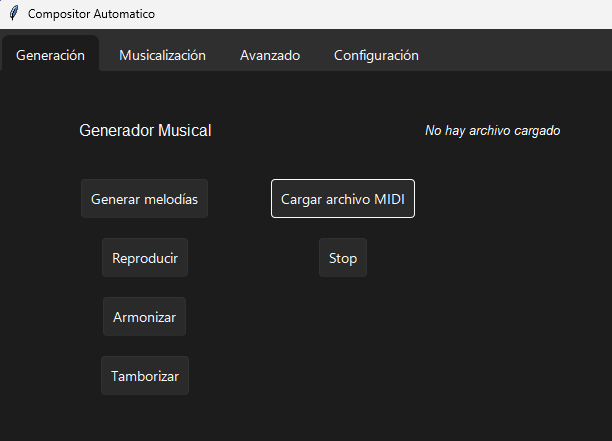
\includegraphics[scale=0.75]{Imagenes/Bitmap/generationTab.png}
    \end{center}
    \caption{Pestaña \generationTabName{}}
    \label{fig:generationTab}
\end{figure}

Esta pestaña reúne las funcionalidades que permite al usuario generar MIDI. Estas funcionalidades se dividen en Generar melodía, Reproducir, Armonizar y Tamborizar.

\begin{itemize}
  \item Generar: Genera MIDI de acuerdo con el generador activo. Para cambiar el generador de midi, ver \nameref{subsec:app:alternarGenerador}.
  \item Reproducir: Reproduce la melodía generada a modo prueba con un sintetizador simple.
  \item Armonizar: Armoniza la melodía generada. Ver el punto \ref{sec:arm:armonia} para más detalle.
  \item Tamborizar: Añade el MIDI asociado a la percusión.
\end{itemize}

\section{Selección de Temática y Sonorización}
\label{sec:SeleccionTematica}

Esta sección describe la pestaña \tematicTabName{} de la aplicación (figura \ref{fig:tematicTab}). 

\begin{figure}[h]
    \begin{center}
        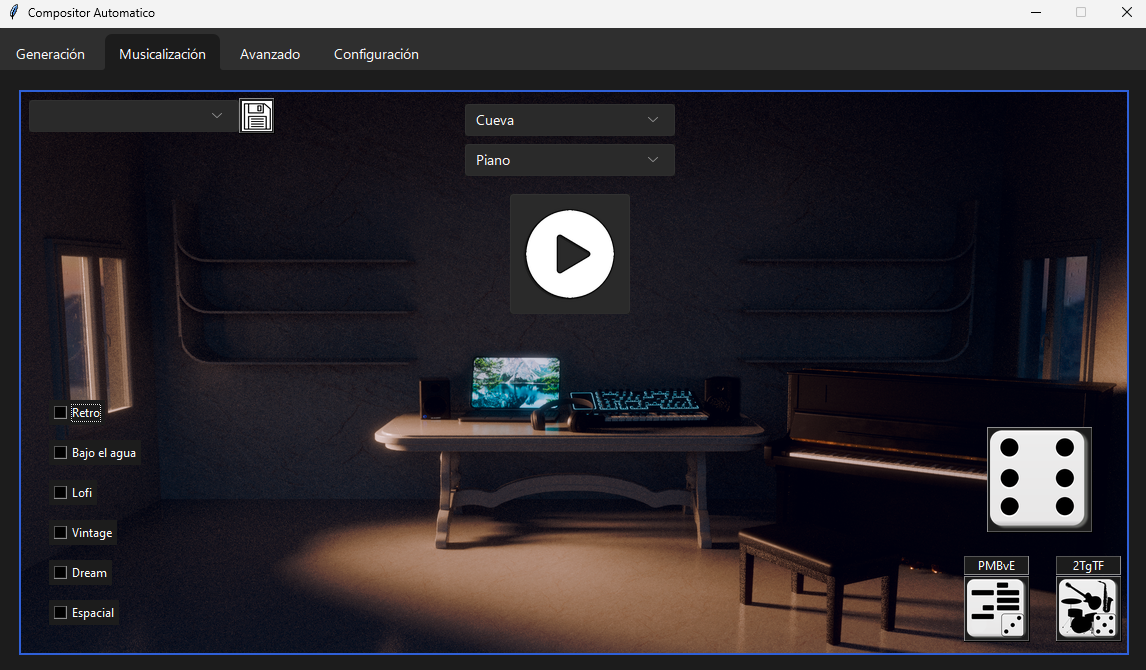
\includegraphics[scale=0.45]{Imagenes/Bitmap/tematicTab.png}
    \end{center}
    \caption{Pestaña \tematicTabName{}}
    \label{fig:tematicTab}
\end{figure}

En esta pestaña disponemos de varias opciones para dirigir la sonorización del MIDI generado en la pestaña \nameref{sec:app:generacionAudio}.

\subsection{Temáticas}
\label{subsec:app:themes}
En la parte superior derecha de la figura \ref{fig:tematicTab}, encontramos un desplegable con las posibles temáticas que se pueden seleccionar. Por defecto viene con la temática Pradera. El estilo del fondo irá cambiando según la temática seleccionada, reflejando la configuración activa. 

En la parte inferior izquierda se encuentran las checkboxex, asociadas a modificadores que alteran la temática de juego. Los cambios en estos modificadores también se ven reflejados en el estilo del fondo de esta pestaña de la aplicación.

\subsection{Semillas}
\label{subsec:app:seed}
En la parte inferior derecha de la figura \ref{fig:tematicTab} se encuentra un botón con forma de dado, el cual genera una semilla aleatoria. Esta semilla será la que se utilice para sonorizar el MIDI una vez se de al botón de reproducir que hay en medio de la pantalla. Una misma semilla generará los mismos instrumentos y pistas siempre que la configuración de \nameref{subsec:app:themes} sea la misma. Es decir, para dos casos de uso donde la semilla sea la misma pero la temática o los modificadores (checkboxes) sean distintos, la generación final de instrumentos y pistas será distinta.

\subsection{Presets}
\label{subsec:app:presets}
Los presets son configuraciones de la pestaña \tematicTabName{} que se guardan dentro de la aplicación. Estas configuraciones albergan el estado de la temática, las checkboxes y la semilla seleccionadas al momento de haberlas guardado. La configuración actual de la pestaña \tematicTabName{} se puede guardar haciendo click en el botón que tiene el icono de la figura \ref{fig:savePresetIcon}.

\begin{figure}[h]
    \begin{center}
        
\includegraphics[scale=0.25]{Imagenes/Bitmap/saveIcon.png}
    \end{center}
    \caption{Icono de guardado}
    \label{fig:savePresetIcon}
\end{figure}

Al pulsar este botón, saltará una ventana solicitando un nombre para el preset (figura \ref{fig:savePresetIcon}). Para crear un nuevo preset, basta con escribir un nombre de preset que no esté registrado ya. Si se introduce un nombre de preset ya registrado, este se sobreescribirá con la información del nuevo estado de la pestaña \tematicTabName{}.

\begin{figure}[h]
    \begin{center}
        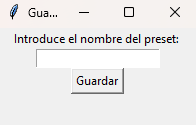
\includegraphics[scale=0.85]{Imagenes/Bitmap/savePresetWindow.png}
    \end{center}
    \caption{Ventana de guardado de preset}
    \label{fig:savePresetWindow}
\end{figure}

Para recuperar un preset, basta con utilizar el desplegable situado en la parte superior izquierda de la pestaña y seleccionar el nombre del preset. Esto actualizará la información de la pestaña con la que había en el momento en el que se guardó ese preset, es decir: temática, checkboxes y semilla.

\section{Modo avanzado}
\label{sec:app:advancedMode}
El objetivo principal de la aplicación es ofrecer a los usuarios una forma sencilla de generar temas musicales. No obstante, está incluida la posibilidad de relizar acciones avanzadas para los usuarios más avezados de la aplicación, así como los que cuentan con conicimiento musical previo.

La posibilidad de editar en REAPER los temas musicales generados por nuestra aplicación sigue existiendo, tal y como está planteado en la sección \nameref{sec:SeleccionTematica}, al pulsar el botón de \textit{Play}. Esto iniciará el ejecutable de REAPER, por lo que en cualquier momento el usuario puede pasar a trabajar directamente en la DAW en lugar de centrarse en nuestra aplicación, permitiendo trabajar con normalidad en REAPER, a partir de los MIDIs e instrumentos generados por \appName{}

En los subapartados siguientes veremos las acciones posibles dentro de la pestaña \advancedTabName{} de la aplicación.

\subsection{Alternar Generador}
\label{subsec:app:alternarGenerador}
Esta opción permite cambiar el modo de generación de la melodía en la pestaña \generationTabName{}. Los generadores disponibles son \nameref{sec:markov-chain}, \nameref{sec:RNR} y \nameref{sec:magenta}. Ver el capítulo \nameref{cap:generacionMusical} para más información acerca de los modos de generacion musical. 

\subsection{Mezclar temáticas}
\label{subsec:app:mixThemes}

\subsection{Mezclar melodías}
\label{subsec:app:mixMelodies}

\section{Configuración}
\label{sec:app:configuration}

La pestaña de configuración permite reorganizar los recursos de la aplicación

\begin{itemize}
    \item Ruta de reaper: La ruta absoluta a reaper es utilizada por la aplicación para poder encontrar el ejecutable de reaper a la hora de reproducir el contenido generado por \appName{}. Por defecto, REAPER se busca en \textit{C:/Program Files/REAPER (x64)/reaper.exe}. Si su ruta absoluta a Reaper es distita a esta, es importante que actualice esta opción para poder usar la app correctamente.
\end{itemize}